\section{Introduction}\label{sec:Intro} 


%The accelerating pace of materials innovation remains a critical challenge in addressing global demands for high-performance structural materials, despite technological advancements in the past few decades. Traditional materials development methods, often characterized by sequential experimentation and empirical adjustments, are inherently limited when faced with the vast and complex design spaces of modern high-entropy alloys (HEAs). 

% Recent advances in closed-loop materials design have transformed how researchers explore complex composition–processing–property spaces \cite{}. the concurrent emergence of high-entropy and compositionally complex alloys has dramatically expanded the design space that materials scientists are willing to explore, offering unprecedented opportunities for property optimization but also introducing combinatorial challenges that make exhaustive exploration impractical. Together, these developments haved motivated data-efficient optimization strategies capable of navigating large, high-dimensional materials spaces while accounting for real experimental constraints \cite{}.


The discovery of advanced structural materials capable of withstanding extreme environments remains a critical challenge in materials science and engineering \cite{}.  Recent advances in closed-loop materials design have transformed how researchers explore complex composition–processing–property spaces in search of such materials  \cite{}. The concurrent emergence and adoption of high-entropy and compositionally complex alloys has dramatically expanded the design space that materials scientists are willing to explore, offering unprecedented opportunities for property optimization but also introducing combinatorial challenges that make exhaustive exploration impractical. Together, these developments have motivated data-efficient optimization strategies capable of navigating large, high-dimensional materials spaces.


 % HEAs, defined by five or more principal elements in near‐equiatomic ratios, offer unprecedented compositional tunability, leading to exceptional combinations of strength, ductility, and thermal stability \cite{Miracle2017, Zhang2014}. However, the sheer number of possible compositions (scaling combinatorially with the number of elements and resolution) creates an intractable search space for conventional methods.

 % Traditional alloy development methods, relying on sequential experimentation and empirical tuning, are inherently slow and often unable to navigate the vast, high‐dimensional compositional spaces characteristic of modern high‐entropy alloys (HEAs) \cite{Yeh2004, Cantor2004}.

Such strategies include integrated computational-experimental frameworks. These frameworks have typically combined high‐throughput (HTP) synthesis and characterization, first‐principles and CALPHAD modeling, and/or closed-loop machine learning (ML)–based optimization \cite{Liu2022, Li2024, Li2017, Zhang2023}. Among these, Bayesian optimization (BO) has shown particular promise for multi‐objective materials design, as it balances exploration of poorly characterized regions with exploitation of promising candidates, all while quantifying uncertainty \cite{Snoek2012,Shahriari2016, Zhang2022, Mamun2025, Hanaoka2022, Arroyave2022}. Recent studies have successfully applied BO to optimize multiple properties simultaneously in refractory HEA structural materials \cite{Khatamsaz2022Multi-objectiveAlloys, Vela2023, Paramore2025}.

Building on these advances, the Batch-Wise Improvement in Reduced Materials Design Space Using a Holistic Optimization Technique (BIRDSHOT) initiative seeks to accelerate the design and discovery of advanced structural materials by combining high-throughput computation, high-throughput experimentation, and active learning strategies within a closed-loop workflow. In our previous work \cite{mulukutla2024illustrating,hastings2025acceleratedmultiobjectivealloydiscovery}, we introduced the foundational BIRDSHOT framework and demonstrated how physics-informed Bayesian optimization coupled with high-fidelity experimentation can efficiently explore vast compositional spaces in high-entropy alloys (HEAs). This effort constituted what we refer to as a "discovery campaign" i.e. a coordinated sequence of model-guided experiments designed to iteratively refine understanding of a material system while converging toward optimal compositions. That prior campaign provided key insights into the relationships between composition, mechanical performance, and phase stability within the Al–V–Cr–Fe–Co–Ni alloy family. Futhermore, this previous campaign proved that multi-objective, closed-loop Bayesian optimization can meaningfully accelerate structural alloy development. A detailed summary of this earlier work, along with distinctions between that campaign and the present study, is provided in the Supplemental Information.

In the present work, we report a new discovery campaign using an updated BIRDSHOT framework that incorporates several methodological and experimental extensions designed to improve robustness, scalability, and exploration efficiency within multi-objective alloy design:

% \subsection{Summary of Prior Work}

% In our previous work, the framework was demonstrated on the Al–V–Cr–Fe–Co–Ni FCC high entropy alloy (HEA) system, targeting three key performance objectives: ultimate tensile strength/yield strength ratio, hardness, and strain rate sensitivity. The study combines several key innovations: (i) initial design space filtering using CALPHAD-based phase stability predictions and property constraints to reduce $\sim$53,000 candidate compositions to 2,437 feasible alloys; (ii) division of the design space based on predicted stacking fault energy (SFE) into low ($<$50~mJ/m$^2$) and high ($>$50~mJ/m$^2$) SFE regimes to explore different deformation mechanisms; (iii) batch Bayesian optimization using an ensemble of Gaussian processes with varying length scales to enable parallel experimentation while avoiding premature convergence; and (iv) Expected Hypervolume Improvement (EHVI) as the acquisition function to guide multi-objective optimization.

% Through five iterative design-make-test-learn loops, each evaluating 8 alloys in parallel, we successfully identified three-objective Pareto sets by exploring only 0.15\% of the feasible design space. The experimental campaign employed vacuum arc melting for synthesis, comprehensive characterization including SEM and XRD for phase verification, quasi-static tensile testing for mechanical properties, and nanoindentation for hardness and strain rate sensitivity measurements. The framework demonstrated significant acceleration over traditional methods, with statistical analysis showing that the observed Pareto set sizes (14 and 15 points for low and high SFE regimes, respectively) had less than 0.5\% probability of occurring through random sampling, validating the effectiveness of the Bayesian approach.


% In other words, this prior work established the foundational principles of this framework within the context of the Al–V–Cr–Fe–Co–Ni system, integrating physics-informed modeling, high-throughput experimentation, and CALPHAD-based phase prediction to optimize for structural performance. This effort provided critical insights into the trade-offs between composition, mechanical properties, and phase stability, while highlighting the benefits of a modular, closed-loop pipeline for accelerated alloy discovery. 



\begin{adjustwidth}{1em}{0em}
\indent \textbf{Risk-Aware Acquisition Strategy}: 
Traditional Bayesian optimization (BO) relies on acquisition functions (e.g., Expected Improvement) that implicitly assume each experiment produces measurable objective values. In practical materials discovery campaigns, however, some candidate alloys lead to so-called ``failed experiments.'' In this context, failure does not indicate poor performance (e.g., low yield strength), but rather that experimental time and resources are expended without obtaining usable property measurements because the alloy cannot be synthesized, processed, or tested under the prescribed conditions. Such outcomes represent a critical risk in closed-loop optimization, where the objective is to maximize information gained per experimental iteration. This risk is amplified by the substantial cost associated with each iteration amounting to several thousands of dollars and significant personnel and instrument time, meaning that even a small fraction of unusable experiments can significantly reduce campaign efficiency and slow convergence of the design loop. Consequently, acquisition decisions must balance potential performance gains with the probability that an experiment will yield actionable data.

Within the present campaign, alloys predicted to form single-phase FCC structures that were subsequently synthesized but observed to contain secondary phases were classified as failed experiments. These materials are expected to introduce processing challenges and, even when mechanically testable, do not provide a consistent basis for comparison within the intended single-phase design space. Incorporating this definition of failure into the acquisition strategy enables a risk-aware search that prioritizes candidates with both high expected performance and a high probability of experimental viability, thereby improving overall information efficiency in the closed-loop workflow. We therefore refine the Bayesian optimization framework by introducing a risk-aware acquisition strategy that actively learns which regions of compositional space are likely to produce failed experiments. The proposed approach probabilistically penalizes high-risk candidates while preserving controlled exploration in uncertain areas. The probabalistic penalty is to ensure a high risk experiment could potentially be explored if and only if it's objective values are predicted to be high. This Bayesian risk awareness is the namesake of the paper.

%In the present campaign, an experiment is classified as failed when an alloy predicted to form a single-phase FCC structure is synthesized but found to contain secondary phases. Such alloys are expected to introduce processing difficulties and, even when mechanically testable, fall outside the intended single phase design space, precluding consistent property comparisons. This definition motivates a feasibility-aware extension to the acquisition strategy: rather than optimizing expected performance alone, the framework must also account for the probability that a candidate will produce actionable data. We therefore augment the BO acquisition function with a learned feasibility model that estimates, for each candidate composition, the likelihood of successful synthesis of single phase FCC alloy. High risk candidates receive a probabilistic penalty during acquisition scoring, reducing their selection priority. Crucially, this penalty is not absolute, a candidate with sufficiently high predicted objective values can still be selected despite elevated risk, preserving controlled exploration in uncertain regions of the compositional space. This risk-aware Bayesian optimization strategy, in which feasibility constraints are learned and embedded directly into the acquisition function, is the namesake of the present work.
\end{adjustwidth}

% \begin{adjustwidth}{1em}{0em}
% \textbf{Diversity-Aware Sampling of an Expanded Alloy Search Space}: In the previous campaign we explored a 6-element alloy space, xxxxxx. In this campaign we explore an 8-element HEA system, Al–V–Cr–Mn–Fe–Co–Ni–Cu. The addition of Mn and Cu into the design space introduces additional capability for tuning ductility, and phase stability, informed by prior experimental insights and domain-specific knowledge. Grid sampling this alloy design space at a resolution of 4 at\% results in xxxxxx alloys. This enumeration is intractable from a data storage, let alone computational tractability. Thus to still explore this large space We deploy a hierarchical, diversity-aware sampling strategy using k-medoids clustering across the ~27,000 alloy feasible space. Alloys are categorized into 37 chemically distinct subsystems, and representative candidates are selected to maximize coverage across these subsystems, enabling effective early-stage learning and simultaneously improving the efficiency of learning in the Bayesian optimization loop.
% \end{adjustwidth}

\begin{adjustwidth}{1em}{0em}
\textbf{Diversity-Aware Sampling of an Expanded Alloy Search Space}: In the previous discovery campaign, we investigated a  6-element HEA compositional space (Al–V–Cr–Fe–Co–Ni). In the present study, the search space is expanded to an 8-element system, Al–V–Cr–Mn–Fe–Co–Ni–Cu. The inclusion of Mn and Cu introduces additional degrees of freedom for tuning ductility and phase stability, as guided by prior experimental insights and domain-specific knowledge.
\end{adjustwidth}

\begin{adjustwidth}{1em}{0em}
Naïve grid sampling of this expanded compositional space at a resolution of 4 at.\% would yield approximately 3.4 million candidate alloys. This enumeration is impractical from both data storage and computational perspectives. To enable tractable exploration while preserving broad chemical coverage, we deploy a hierarchical, diversity-aware sampling strategy based on k-medoids clustering across the $\sim$27{,}000-alloy feasible space (i.e. alloys within the Al–V–Cr–Mn–Fe–Co–Ni–Cu that are predicted to be single phase FCC). Alloys are partitioned into 37 chemically distinct subsystems, from which representative candidates are selected to maximize diversity and compositional coverage. This approach improves early-stage learning efficiency and enhances exploration within the Bayesian optimization loop by prioritizing chemically informative samples rather than densely sampling redundant regions of the design space.
\end{adjustwidth}

% \textbf{Hierarchical, Diversity-Aware Sampling}: We deploy a hierarchical, diversity-aware sampling strategy using k-medoids clustering across the ~27,000 alloy feasible space. Alloys are categorized into 37 chemically distinct subsystems, and representative candidates are selected to maximize coverage across these subsystems, enabling effective early-stage learning and simultaneously improving the efficiency of learning in the Bayesian optimization loop.


 %The integration of advanced characterization techniques, including high strain rate nanoindentation, high-strain-rate testing through split hopkinson bar testing (SPHB), and dynamic small punch testing (SPT), alongside simulation-based metric of modeled depth of penetration, enables a comprehensive and scalable platform for multi-objective, risk-aware high-throughput alloy discovery.

     %\item Dynamic Small Punch Testing (SPT) using a modified SHPB-based setup for impact-relevant testing on small-scale samples, and %Check if we want to include SPT as it is not used in the BO loop

     

\begin{adjustwidth}{1em}{0em}
\textbf{Comprehensive, High-Throughput Characterization}: Five material objectives are evaluated in this work: Yield Strength (YS), Ultimate Tensile Strength to Yield Strength Ratio (UTS/YS), strain at UTS, Ratio of Dynamic and Quasi-Static Strength Measures (DS/QS), and Depth of Penetrtion (DoP). Mechanical performance is assessed through a coordinated high-throughput workflow integrating experimental testing with physics-based modeling. The characterization framework includes:
\begin{itemize}
    \item Tensile testing to quantify YS, UTS/YS, and strain at UTS.
    \item Quasistatic and high-strain-rate nanoindentation to probe rate-dependent deformation behavior.
    \item SHPB experiments to evaluate bulk dynamic response and provide calibration data for strain-rate–dependent constitutive modeling.
    \item Finite-element ballistic impact simulations implemented in ABAQUS/Explicit using calibrated Cowper--Symonds viscoplastic models to compute DoP.
\end{itemize}
Together, these measurements provide complementary insight into quasi-static strength, strain-rate sensitivity, and modeled impact resistance across the candidate alloy space.
\end{adjustwidth}

To enable experimentation at scale, we established a high-throughput sample preparation workflow incorporating automated polishing, laser marking for traceability, and large-batch fixturing supporting up to 48 samples per run. Custom Python and ImageJ pipelines were developed to automate image analysis, contact-area measurement, and extraction of data from encrypted binary outputs, substantially reducing manual intervention while improving consistency, data fidelity, and reproducibility.

These capabilities transform the present study into a scalable testbed for autonomous, closed-loop alloy discovery, where experimental measurements directly inform model refinement and candidate selection across successive iterations. By combining exploration of high-dimensional compositional spaces with risk-aware Bayesian optimization, advanced mechanical characterization, and simulation-informed modeling, this work establishes an integrated, end-to-end workflow for the accelerated design of structural alloys targeting extreme environments.

The complete BIRDSHOT framework—encompassing computational design, synthesis, characterization, and simulation—is summarized in Fig.~\ref{fig:full_framework}, illustrating the multi-stage feedback loop that links physics-based modeling with high-throughput experimentation. This integrated platform enables multi-objective, risk-aware materials discovery while capturing both quasi-static and dynamic performance metrics within a unified campaign.

In summary, this paper presents the design rationale, methodologies, and outcomes of a closed-loop alloy design study that integrates active learning, mechanistic modeling, and scalable experimentation. The resulting workflow demonstrates a practical pathway toward accelerated discovery of high-performance structural alloys, addressing real-world constraints such as phase stability, manufacturability, and experimental throughput while advancing autonomous materials development.


% To enable these experiments at scale, we developed a high-throughput sample preparation workflow, including automated polishing, laser marking for traceability, and large-batch fixturing to support up to 48 samples per run. Additionally, we built custom Python and ImageJ scripts to automate image analysis, contact area measurement, and data extraction from encrypted binary outputs—reducing manual intervention and experimental variability while improving data quality and reproducibility.

% Together, all of these components make this study a more comprehensive and scalable testbed for autonomous, closed-loop alloy discovery, where data from physical experiments directly inform model refinement and candidate selection in subsequent iterations. The combination of high-dimensional composition space exploration, risk-aware Bayesian optimization, advanced mechanical testing, and simulation-informed modeling provides a unified, end-to-end platform for accelerating the design of structural alloys tailored for extreme environments.

% The entire BIRDSHOT framework, including all computational, synthesis, characterization, and simulation steps involved in this study, is summarized in Fig.~\ref{fig:full_framework}, providing an overview of the integrated, multi-stage closed loop materials discovery workflow. Together, these improvements enable a multi-objective, risk-aware, high-throughput materials discovery platform capable of navigating a high-dimensional compositional space while capturing a rich set of mechanical performance metrics under both quasi-static and dynamic loading conditions.


% In summary, this paper presents the design rationale, computational and experimental methodologies, and findings from the study, highlighting the integration of active learning, mechanistic modeling, and high-throughput experimentation. The case study explored using this framework aims to accelerate discovery of high performance alloys suitable for demanding structural applications. These improvements position our framework as a scalable and robust testbed for closed-loop materials discovery, while also addressing practical constraints related to phase formation, manufacturability, and experimental throughput.

\begin{figure}[H]
    \centering
    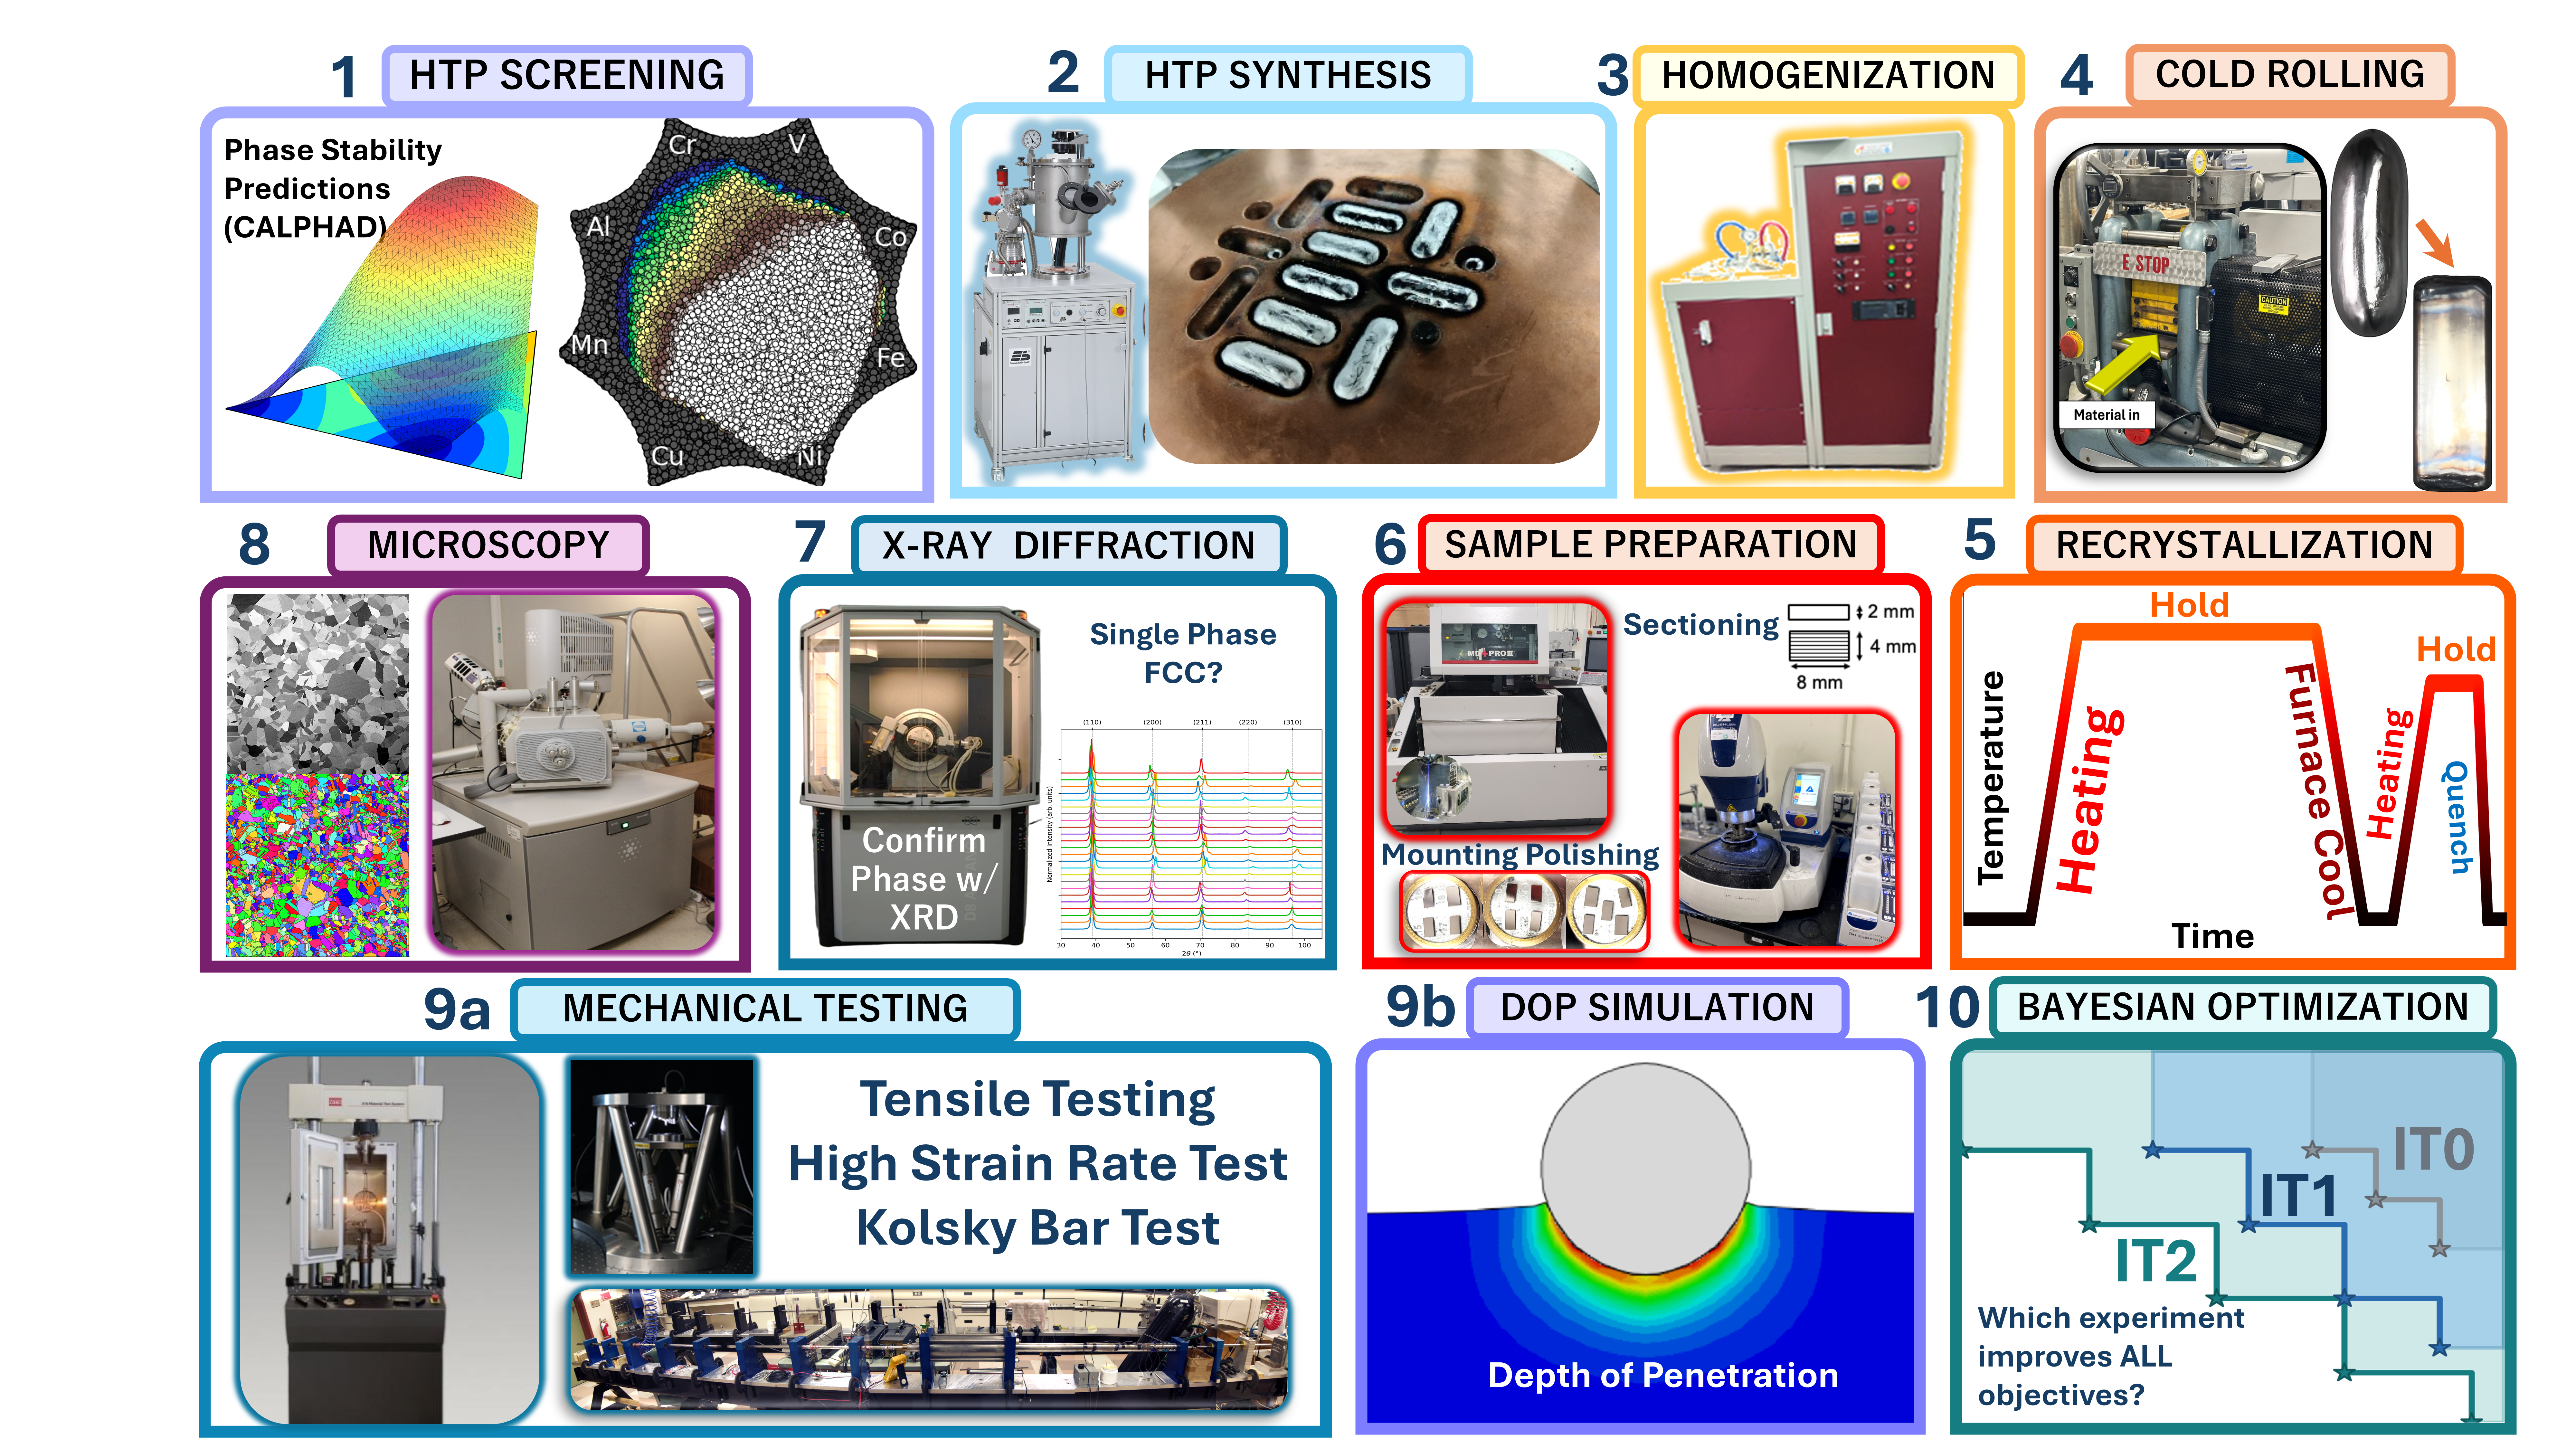
\includegraphics[width=0.9\linewidth]{Figures/C2_Schematic.png}
    \caption{Comprehensive BIRDSHOT workflow showing all computational, synthesis, characterization, and simulation steps. The sequential diagram highlights the complexity and interdependence of processes in this multi-stage materials discovery campaign.}
    \label{fig:full_framework}
\end{figure}















